\section{What changes when an agent improves}\label{sec:C30:01}
An improvement claim is incomplete until the mutable object is identified. A system can change its active context, persistent records, procedural skills, execution harness, environment curriculum, verifier, or model parameters. These changes have different costs, failure modes, and transfer requirements. Updating a skill index changes which procedures are retrieved; updating a model changes how every retrieved procedure is interpreted. A harness search can improve a frozen policy without producing any new parametric capability. Distinguishing the update target is necessary for attributing a result and for deciding whether the resulting state can be safely reused.

Let $\xi=(\theta,h,m,v,e)$ collect model parameters, harness configuration, memory, verifier, and environment-generation rules. An improvement operator $\mathcal I_\omega$ proposes a new configuration from an evidence set $D$ and resource budget $B$:
\begin{equation}
 \xi'=\mathcal I_\omega(\xi,D;B).
\end{equation}
An accepted update is a decision made by an acceptance rule, not a mathematical guarantee that quality increased. Let $\mathcal U_\omega(\xi,D;B)$ denote the complete proposal-and-acceptance procedure: it returns the selected configuration, or the unchanged incumbent when all proposals are rejected. Its budget includes the acceptance computation. The relevant quantity is held-out utility $J(\xi;\mathcal D)$ under a declared task population and operational cost boundary. An update can improve its selection score while degrading $J$ if it exploits grading weaknesses, changes the distribution, or consumes more unreported resources.

Recursive self-improvement adds a second question: does the change improve the process that will generate later changes? Define executor utility $J(\xi)$ and improver utility
\begin{equation}
 K(\omega;\xi,B)=
 \mathbb E\left[J(\mathcal U_\omega(\xi,D;B))-J(\xi)\right].
 \label{eq:c30:improver}
\end{equation}
The expectation includes task sampling, proposal randomness, evaluation noise, and the acceptance policy. A positive change in $J$ does not imply a positive change in $K$. A patch can solve a particular recurring failure while making the next search process less diverse, more expensive, or more vulnerable to its evaluator. Evidence for improved execution and evidence for improved improvement must therefore be reported separately.

\begin{table}[!htbp]
\centering
\caption{Mutable adaptation targets and distinct validation obligations.}\label{tab:C30:targets}
\begin{tabular}{L{0.22\linewidth}L{0.31\linewidth}L{0.34\linewidth}}

\toprule Update target & Observable mutation & Distinct validation obligation\\\midrule
Context & Tokens selected, compressed, or reconstructed & Decision preservation and correct behavior-policy conditioning.\\
Memory & Facts, episodes, links, or retrieval indexes & Validity, influence, task-order effects, and deletion propagation.\\
Skills & Procedures and their applicability conditions & Transfer, compatibility, and permission revalidation.\\
Harness & Prompts, control flow, tools, middleware & Resource-matched transfer and crash/recovery behavior.\\
Model & Weights, adapters, or learned routers & Held-out capability, regressions, and state migration.\\
Verifier & Tests, rubrics, judges, or calibration & Independent false-acceptance and false-rejection evidence.\\
Environment & Tasks, simulations, or curricula & Grounding, coverage, difficulty, and leakage.\\
\bottomrule
\end{tabular}
\end{table}

The taxonomy is operational. A method may update several targets, but it should identify the order and dependency of those updates. Reflection-based text memories, for example, can alter subsequent actions without changing weights. Reflexion provides an early concrete mechanism for this form of adaptation, whereas parametric post-training changes the conditional model itself~\cite{shinn2023reflexion}. Calling both learning is reasonable only if the analysis retains their different persistence, compute, and generalization properties.


% SCIENTIFIC_FIGURE_C30
Figure~\ref{fig:C30:overview} separates the executor, the improver, and the independent evaluation of a frozen executor.
\begin{figure}[!htbp]
\centering
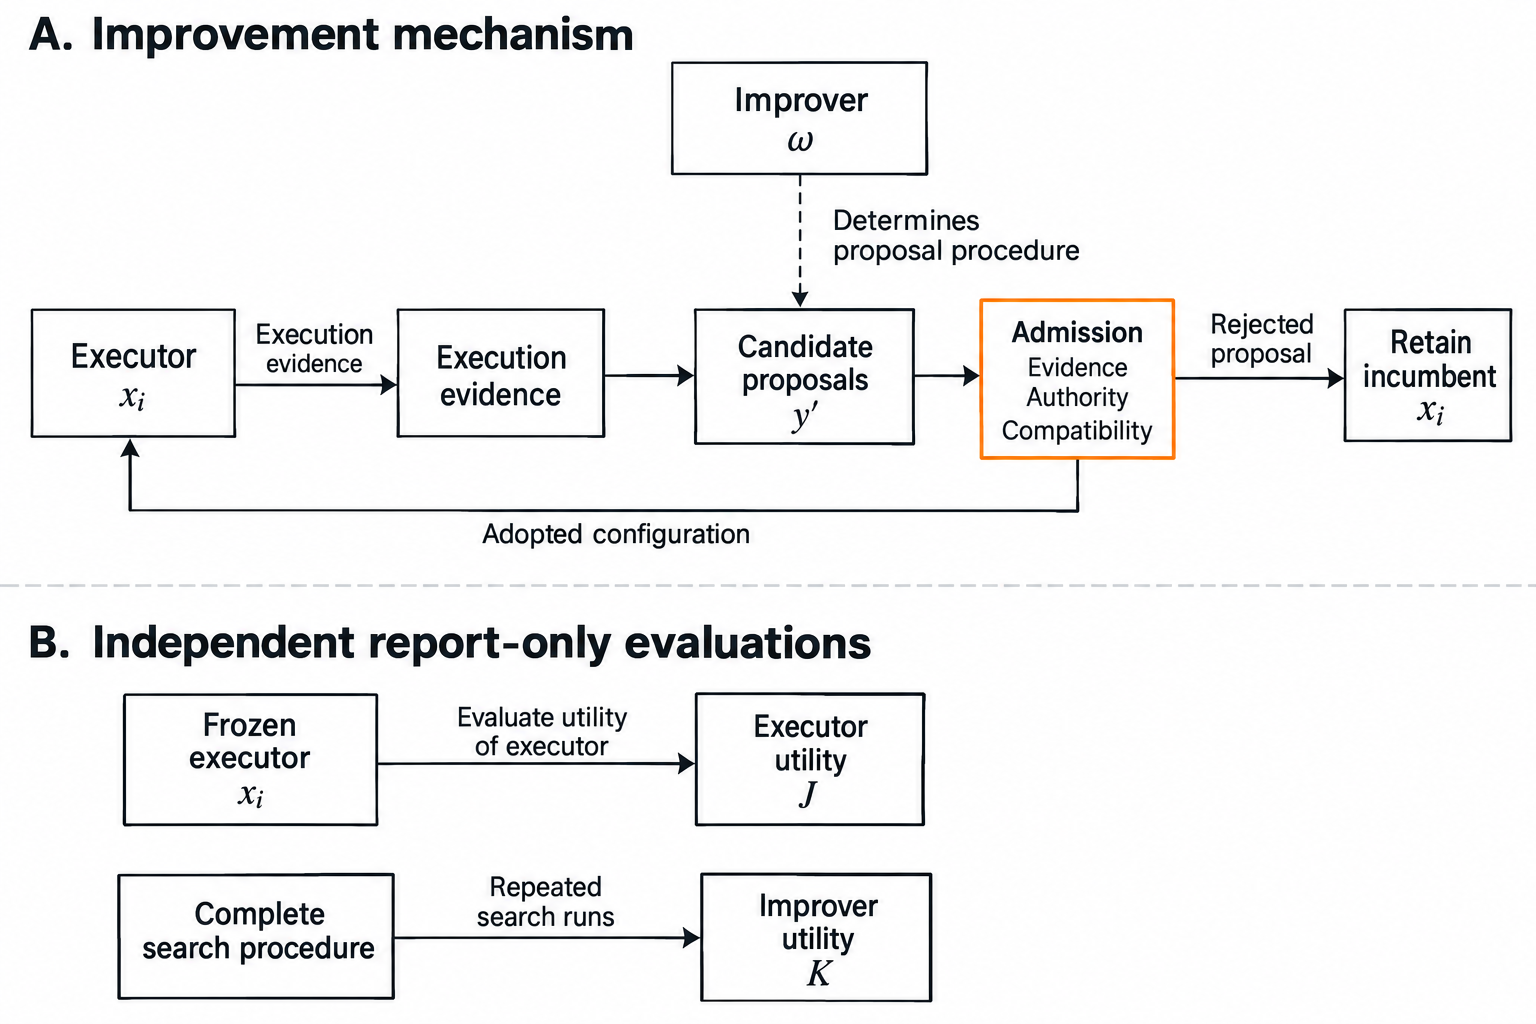
\includegraphics[width=\linewidth]{book/figures/assets/F30review.png}
\caption{Executor utility $J$ and the expected gain $K$ of the complete improvement procedure are different estimands. Here $x_i$ labels the incumbent executor configuration, $y^\prime$ a proposal, and $\omega$ the improver. Adoption also depends on evidence, authority and compatibility. Independent outer-loop runs and complete search costs are needed to assess improvement; a selected executor score cannot substitute for that assessment.}
\label{fig:C30:overview}
\end{figure}
